\documentclass[pdf]{beamer}

\usetheme{CambridgeUS}
\usepackage[utf8x]{inputenc}
\usepackage{listings}
\lstset{basicstyle={\footnotesize}}
\usepackage{graphicx}

\mode<presentation>{}
\title{Building an LLVM Backend}
\subtitle{LLVM 2014 tutorial}
\author{Fraser Cormak \\ Pierre-Andre Saulais \\ Codeplay Software \\ @codeplaysoft}

\begin{document}

%%%%%%%%%%%%%%%%%%%%%%%%%%%%%%%%%%%%%%%%%%%%%%%%%%%%%%%%%%%%%%%%%%%%%%%%%%%%%%%%

\begin{frame}
\titlepage
\end{frame}

%%%%%%%%%%%%%%%%%%%%%%%%%%%%%%%%%%%%%%%%%%%%%%%%%%%%%%%%%%%%%%%%%%%%%%%%%%%%%%%%

\begin{frame}{Introduction}

\begin{itemize}
    \item Yet another talk about creating a LLVM target?
    \item LLVM backend crash course, for beginners
    \begin{itemize}
        \item How-tos and tips
        \item Solution to common problems
    \end{itemize}  
    \item Example target created for this tutorial
    \begin{itemize}
        \item Can be used to see how LLVM works
        \item Can be used as a skeleton to bootstrap new target
    \end{itemize}
\end{itemize}

\end{frame}

%%%%%%%%%%%%%%%%%%%%%%%%%%%%%%%%%%%%%%%%%%%%%%%%%%%%%%%%%%%%%%%%%%%%%%%%%%%%%%%%

\begin{frame}{Overview}

\begin{itemize}
    \item Part 1: Background
    \item Part 2: Creating your own target
    \item Part 3: How-tos for specific tasks
    \item Part 4: Troubleshooting and tips
\end{itemize}

\end{frame}

%%%%%%%%%%%%%%%%%%%%%%%%%%%%%%%%%%%%%%%%%%%%%%%%%%%%%%%%%%%%%%%%%%%%%%%%%%%%%%%%

\section{Part 1: Background}

\begin{frame}{Part 1}

Background

\end{frame}

%%%%%%%%%%%%%%%%%%%%%%%%%%%%%%%%%%%%%%%%%%%%%%%%%%%%%%%%%%%%%%%%%%%%%%%%%%%%%%%%

\begin{frame}{What you need to start}

\begin{itemize}
    \item Know a little bit about LLVM IR: \\ \url{llvm.org/docs/LangRef.html}
    \item xdot.py to visualize graphs when debugging: \\ \url{github.com/jrfonseca/xdot.py}
    \item Check out and build our LLVM repo from GitHub: \\ \url{github.com/frasercrmck/llvm-leg}
    \item This informative and well-presented talk!
\end{itemize}

\end{frame}

%%%%%%%%%%%%%%%%%%%%%%%%%%%%%%%%%%%%%%%%%%%%%%%%%%%%%%%%%%%%%%%%%%%%%%%%%%%%%%%%

\begin{frame}{Example target: LEG}

\begin{itemize}
    \item Simple, RISC-like architecture
    \begin{itemize}
        \item Very small subset of ARM
    \end{itemize}
    \item 12 integer registers (32-bit)
    \begin{itemize}
        \item r0, r1, ..., r9, sp (stack pointer), lr (return address)
    \end{itemize}
    \item Instructions:
    \begin{itemize}
        \item 32-bit arithmetic (add, subtract, multiply, mad)
        \item 32-bit register move, 16-bit constant moves
        \item load, store, branch, branch and link
    \end{itemize}
\end{itemize}

\end{frame}

%%%%%%%%%%%%%%%%%%%%%%%%%%%%%%%%%%%%%%%%%%%%%%%%%%%%%%%%%%%%%%%%%%%%%%%%%%%%%%%%

\begin{frame}[fragile]{Calling convention for LEG}

\begin{itemize}
    \item How values are passed to/from a function
    \item Arguments in r0 (1st), r1 (2nd), …, r3 (4th)
    \begin{itemize}
        \item Further arguments passed on the stack
    \end{itemize}
    \item Return value in r0
\end{itemize}

\begin{block}{ex1.c}
\begin{lstlisting}
int foo(int a, int b) {
    int result = a + b;   // r0 + r1
    return result;        // r0
}
\end{lstlisting}
\end{block}

\begin{block}{ex1.s}
\begin{lstlisting}
.foo:
    add r0, r0, r1
    b lr
\end{lstlisting}
\end{block}

\end{frame}

%%%%%%%%%%%%%%%%%%%%%%%%%%%%%%%%%%%%%%%%%%%%%%%%%%%%%%%%%%%%%%%%%%%%%%%%%%%%%%%%

\begin{frame}{The big picture}

\begin{itemize}
    \item Pipeline structure of the backend:
    \begin{itemize}
        \item IR → SelectionDAG → MachineDAG  → MachineInstr → MCInst
    \end{itemize}
    \item Transforms your program many times
    \begin{itemize}
        \item Same program, few different representations
        \item Different instruction namespaces
        \item Check it out (IR and MI only):
        \begin{itemize}
            \item $llc foo.ll -print-after-all 2>\&1 > foo.log$
        \end{itemize}
    \end{itemize}
\end{itemize}

\end{frame}

%%%%%%%%%%%%%%%%%%%%%%%%%%%%%%%%%%%%%%%%%%%%%%%%%%%%%%%%%%%%%%%%%%%%%%%%%%%%%%%%

\begin{frame}[fragile]{A look at an IR module}

\begin{itemize}
    \item High-level, linear representation
    \item Typed values, no registers
    \item Target-agnostic
    \begin{itemize}
        \item Exceptions: data layout, triple, intrinsics
    \end{itemize}
\end{itemize}

\begin{block}{ex1.ll}
\begin{lstlisting}
target datalayout = "e-m:e-p:32:32-i1:8:32-i8:8:32-i16:16:32-i64:32-f64:32-a:0:32-n32"
target triple = "leg"

define i32 @foo(i32 %a, i32 %b) {
    %c = add nsw i32 %a, %b
    ret i32 %c
}
\end{lstlisting}
\end{block}

\end{frame}

%%%%%%%%%%%%%%%%%%%%%%%%%%%%%%%%%%%%%%%%%%%%%%%%%%%%%%%%%%%%%%%%%%%%%%%%%%%%%%%%

\begin{frame}{A look at a SelectionDAG graph}

\begin{columns}[t]
\column{.5\textwidth}
    \begin{itemize}
        \item Graph representation
        \item Operations as nodes
        \begin{itemize}
            \item Mostly target-agnostic
            \item LEGISD (ISD) namespace
        \end{itemize}
        \item Dependencies as edges
        \begin{itemize}
            \item Data
            \item Order (“chain”)
            \item Scheduling (“glue”)
        \end{itemize}
        \item Typed values
    \end{itemize}
\column{.5\textwidth}
    \begin{block}{}
        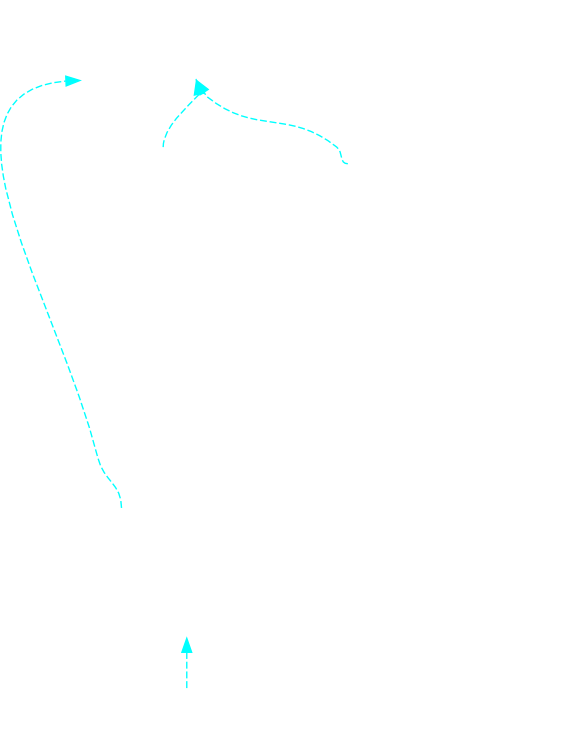
\includegraphics[width = 0.8\textwidth]{examples/ex1-entry-selection-dag.png}
    \end{block}
\end{columns}

\end{frame}

%%%%%%%%%%%%%%%%%%%%%%%%%%%%%%%%%%%%%%%%%%%%%%%%%%%%%%%%%%%%%%%%%%%%%%%%%%%%%%%%

\begin{frame}{A look at a MachineDAG graph}

\begin{columns}[t]
\column{.5\textwidth}
    \begin{itemize}
        \item Very similar to SelectionDAG
        \item Instructions as nodes
        \begin{itemize}
            \item Result of instruction selection
            \item LEG namespace
        \end{itemize}
        \item Similar dependencies
        \item Similar types
    \end{itemize}
\column{.5\textwidth}
    \begin{block}{}
        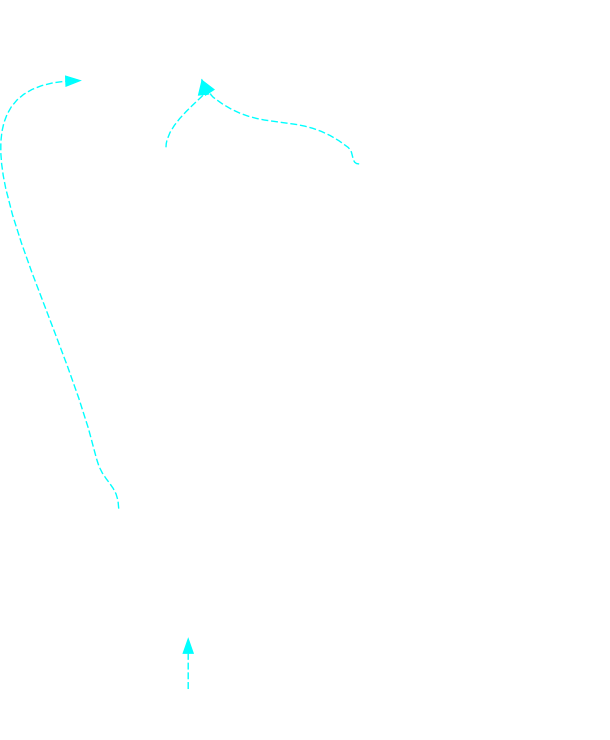
\includegraphics[width = 0.8\textwidth]{examples/ex1-entry-machine-dag.png}
    \end{block}
\end{columns}

\end{frame}

%%%%%%%%%%%%%%%%%%%%%%%%%%%%%%%%%%%%%%%%%%%%%%%%%%%%%%%%%%%%%%%%%%%%%%%%%%%%%%%%

\begin{frame}{Before and after ISel}

\begin{columns}[t]
\column{.5\textwidth}
    \begin{block}{Before}
        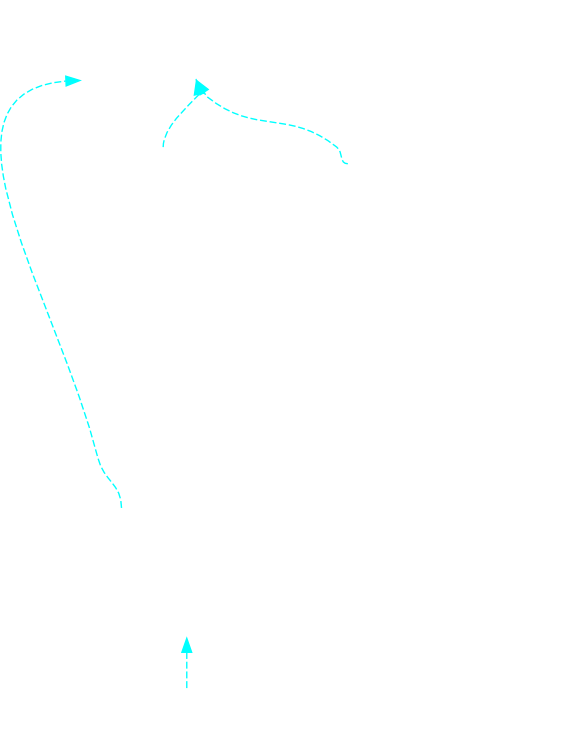
\includegraphics[width = 0.75\textwidth]{examples/ex1-entry-selection-dag.png}
    \end{block}
\column{.5\textwidth}
    \begin{block}{After}
        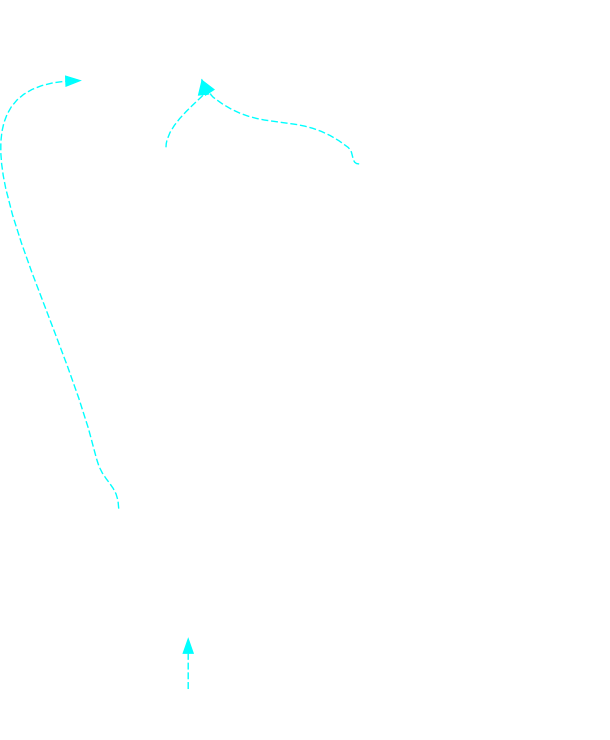
\includegraphics[width = 0.8\textwidth]{examples/ex1-entry-machine-dag.png}
    \end{block}
\end{columns}

\end{frame}

%%%%%%%%%%%%%%%%%%%%%%%%%%%%%%%%%%%%%%%%%%%%%%%%%%%%%%%%%%%%%%%%%%%%%%%%%%%%%%%%

\begin{frame}[fragile]{A look at an IR module}

\begin{itemize}
    \item Untyped, uses register classes instead
    \item Target-specific instructions (LEG namespace)
    \begin{itemize}
        \item Few exceptions (TargetOpcode namespace)
    \end{itemize}
\end{itemize}

\begin{block}{ex1-mi.txt}
\begin{lstlisting}
BB#0: derived from LLVM BB %entry
    Live Ins: %R0 %R1

	%R0<def> = ADDrr %R0<kill>, %R1<kill>  ; %R0, %R1, %R2: GRRegs

    Successors according to CFG: BB#1
\end{lstlisting}
\end{block}

\end{frame}

\end{document}
